\documentclass[12pt]{article}
\frenchspacing
\usepackage[utf8x]{inputenc}
\usepackage[T2A]{fontenc}
\usepackage{amsmath}
\usepackage{amsfonts}
\usepackage{amssymb}
\usepackage[russian]{babel}
\usepackage{graphicx}
\usepackage{hyperref}
\usepackage{multirow}
\usepackage[left=2cm,right=2cm,top=2cm,bottom=2cm,bindingoffset=0cm]{geometry}
\author{Рашковецкий М.М., группа 526т}
\date{\today}
\title{Лабораторная работа 2.2.1\\Исследование взаимной диффузии газов}

\newcommand{\degC}{^\circ \text{C}}
\newcommand{\fref}[1]{рис. \ref{#1}}

\begin{document}
	\maketitle
	
	{\parindent=1cm \hangindent=1cm \parskip=0.5cm
	{\bfseries Цель работы:} регистрация зависимости концентрации гелия в воздухе от времени с помощью датчиков теплопроводности при разных начальных давлениях смеси газов; определение коэффициента диффузии по результатам измерений.
	
	\hangindent=1cm
	{\bfseries Оборудование и материалы:} измерительная установка; форвакуумный насос; баллон с гелием; манометр; источник питания; магазин сопротивлений; гальванометр; секундомер.\par}
	\section*{Краткая теория}
	
	\indent Диффузия --- самопроизвольное перемешивание молекул вследствие их хаотичного теплового движения. При перемешивании молекул разного сорта говорят о взаимной (коцентрационной) диффузии. Для наблюдения диффузии требуется равенство давлений в системе, иначе возникнет просто течение газа как целого.
	
	В системе из двух компонентов плотность потока обоих веществ определяется законом Фика:
	\begin{equation}
		\label{eq:Fick_law}
		j_a=-D_{ab}\frac{\partial n_a}{\partial x}, j_b=-D_{ba}\frac{\partial n_b}{\partial x},
	\end{equation}
	где $D_{ab}=D_{ba}=D$ --- коэффициент взаимной диффузии компонентов, $j_{a,b}$ --- соотв. плотности потоков.
	
	В работе исследуется диффузия примеси гелия на фоне воздуха, изменением концентрации воздуха мы пренебрегаем и впредь, если не оговорено обратного, под $n$ будем понимать концентрацию гелия.
	
	В работе используются два сосуда с объёмами $V_1$ и $V_2$, соединённые трубкой длины $l$ и сечения $S$. Обозначим концентрации гелия в них $n_1$ и $n_2$ соотв. Если процесс выравнивания концентраций происходит достаточно медленно, то поток частиц через все сечения трубки одинаков, поэтому градиент концентраций вдоль ней равномерный и поток равенство
	\begin{equation}
		\label{eq:stream_tube}
		J=-DS\frac{n_1-n_2}{l}.
	\end{equation}
	
	Для изменений концентраций справедливо
	\begin{equation}
		\label{eq:conc_change}
		V_1 dn_1=-V_2 dn_2 = Jdt=-DS \frac{n_1-n_2}{l} dt.
	\end{equation}
	
	Разделим на $dt$:
	\begin{equation}
		\label{eq:conc_change_by_t}
		V_1 \frac{dn_1}{dt}=-DS \frac{n_1-n_2}{l} dt, V_2 \frac{dn_2}{dt}=DS \frac{n_1-n_2}{l} dt.
	\end{equation}
	
	Разделим на $V_{1,2}$ и вычтем одно из другого, тогда
	\begin{equation}
		\label{eq:conc_diff_change_by_t}
		\frac{dn_1-dn_2}{dt}= -DS \frac{n_1-n_2}{l} \left( \frac{1}{V_1} + \frac{1}{V_2} \right).
	\end{equation}
	
	Для разности концентраций $\Delta n=n_1-n_2$, тогда уравнение легко интегрируется:
	\begin{equation}
		\label{eq:conc_by_t_sol}
		\Delta n=\Delta n_0 e^{-t/\tau},
	\end{equation}
	где
	\begin{equation}
		\label{eq:tau}
		\tau=\frac{V_1 V_2}{V_1+V_2} \frac{l}{SD}.
	\end{equation}
	
	Квазистационарное приближение применимо, если время $\tau$ много больше характерного времени диффузии частицы вдоль трубки:
	\begin{equation}
		\label{eq:quasistat_use}
		t_\text{диф} \sim \frac{l^2}{D} \ll \tau.
	\end{equation}
	
	Для измерений концентраций используются датчики теплопроводности, состоящие из тонкой проволоки радиусом $r_\text{пр}$, нагреваемой током и протянутой вдоль оси стеклянного цилиндра радиусом $R_\text{ц}$. Тепло от проволоки к цилиндру передаётся в основном за счёт теплопроводности, мощность передачи равна
	\begin{equation}
		\label{eq:transf_pow}
		Q=\varkappa \frac{2\pi L}{\ln(R_\text{ц}/r_\text{пр})}(T_1-T_2),
	\end{equation}
	где $\varkappa$ --- теплопроводность, $L$ --- длина нити, $T_1$, $T_2$ --- температуры проволочки и стенки. При заданном режиме нагревания температура и соотв. сопротивление проволоки определяется теплопроводностью газа, зависящей от его состава.
	
	Для измерения разности концентраций используется мостовая схема. Мост балансируется при помощи сопротивлений при нулевой разности концентраций, при другой разности возникает разбалансировка моста, зависящая от $\Delta n$.
	
	Вообще зависимость теплопроводности от состава смеси газов сложна, но в первом приближении можно ожидать линейность, что подтверждается экспериментально: при разности концентраций 15\% поправка к линейности всего 0,5\%, чего нам хватит.
	
	Тогда с достаточной точностью показания приборов будут меняться по формуле, аналогичной \eqref{eq:conc_by_t_sol}:
	\begin{equation}
		\label{eq:meas_by_t}
		N=N_0 e^{-t/\tau}.
	\end{equation}
	
	Некоторые особенности методики.
	\begin{enumerate}
		\item Для устранения конвекции датчик выполнен в форме длинной стеклянной трубки с платиновой нитью. Внутренняя часть датчика сообщается с сосудом отверстием такого размера, что скорость диффузии между сосудами намного меньше, чем между сосудом и датчиком. Т.о., состав газа в датчике почти совпадает с составом в сосуде.
		\item В силу неполного обмена энергией между молекулами газа и проволокой возле её поверхности возникает температурный скачок, из-за этого, а также из-за того, что датчики немного разные, баланс немного зависит от давления. Поэтому рекомендуется балансировать мост при каждом давлении в чистом воздухе.
	\end{enumerate}
	
	\section*{Установка}
	
	\begin{figure}[h!]
	\caption{Схема установки}
	\label{fig:scheme}
	\begin{center}
	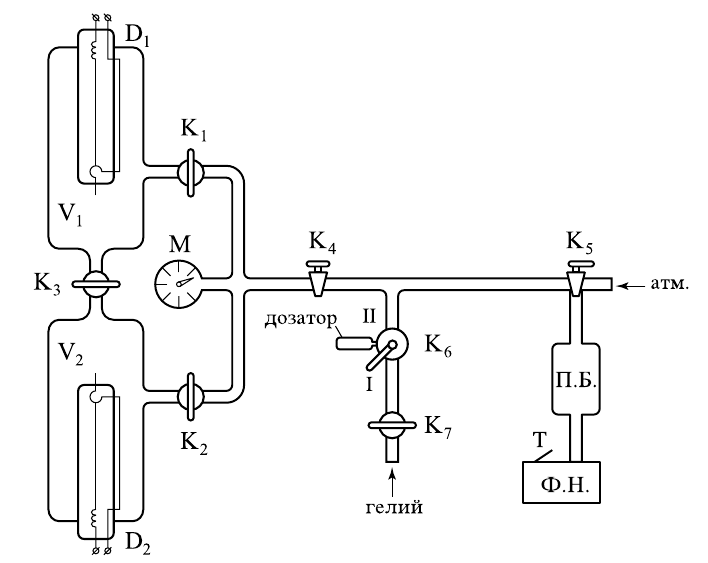
\includegraphics[scale=.6]{scheme.png}
	\end{center}
	\end{figure}
	
	Схема установки изображена на \fref{fig:scheme}. Она состоит из двух сосудов $V_1$ и $V_2$, соединённых краном $K_3$, форвакуумного насоса Ф.Н. с выключателем Т, манометра М и системы напуска гелия, включающей краны $K_6$ и $K_7$. Кран $K_5$ позволяет соединять насос с установкой или атмосферой, предохранительный баллон П.Б. защищает этот кран и установку от попадания масла из насоса при неправильной эксплуатации.
	
	На \fref{fig:scheme2} приведена схема электрических соединений.
	
	\begin{figure}[h!]
	\caption{Мостовая схема с датчиками теплопроводности}
	\label{fig:scheme2}
	\begin{center}
	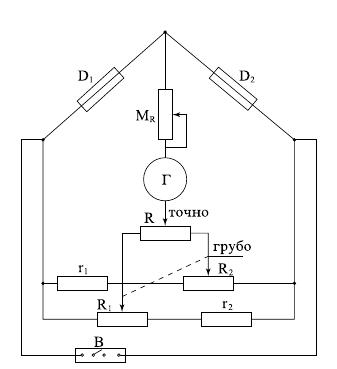
\includegraphics[scale=.6]{scheme2.png}
	\end{center}
	\end{figure}
	
	В трубопроводе давление гелия больше атмосферного. Это нужно, чтобы несмотря на утечки, гелий оставался там без примесей воздуха. Система напуска гелия обычно имеет утечки, поэтому для его сохранения и предотвращения протекания гелия в установку кран $K_7$ обычно закрыт.
	
	Устройство крана $K_6$ показано на \fref{fig:scheme3}. Когда рычажок находится в положении I, дозатор (малый объём) наполняется до давления гелия в трубопроводе, затем рычажок переводится в положение II и гелий из дозатора перетекает в установку. Эту процедуру следует повторять, пока не создастся требуемое давление гелия.
	
	\begin{figure}[h!]
	\caption{Кран $K_6$}
	\label{fig:scheme3}
	\begin{center}
	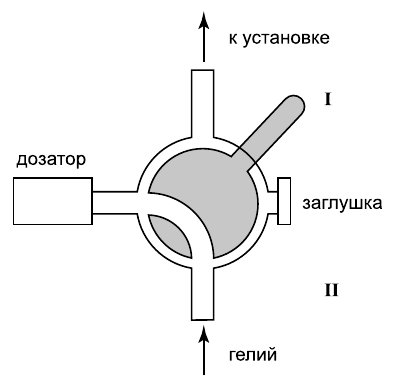
\includegraphics[scale=.5]{scheme3.png}
	\end{center}
	\end{figure}
	
	\section*{Ход работы}
	
	\begin{enumerate}
		\item Записал параметры установки: $V_1=(800\pm 5) \,\text{см}^3$, $V_2=(800\pm 0{,}5) \,\text{см}^3$, $L/S=(11\pm 1) \,\text{см}^{-1}$.
		\item Включил питание электрической схемы, включил компьютер, открыл краны $K_1$, $K_2$, $K_3$.
		\item С помощью форвакуумного насоса очистил установку от всех газов, откачав её до давления $\sim$0,1 торр. \label{exp_loop_begin}
		\item Напустил воздух до рабочего давления, сбалансировал мост.
		\item Заполнил установку рабочей смесью (в $V_1$ --- смесь воздуха и гелия, в $V_2$ --- воздух):
		\begin{enumerate}
			\item Откачал установку.
			\item Изолировал $V_2$.
			\item Заполнил $V_1$ гелием до $0{,}2P_\text{рабочее}$.
			\item Изолировал $V_1$.
			\item Откачал гелий из патрубков форвакуумным насосом.
			\item Соединил с остальной установкой $V_2$.
			\item Наполнил $V_2$ воздухом до $1{,}5P_\text{рабочее}$.
			\item Закрыл $K_4$.
			\item Открыл $K_2$ на 20 с, затем закрыл $K_1$, $K_2$.
		\end{enumerate}
		\item Открыл $K_3$ и запустил измерения на компьютере.
		\item Подождал, пока показания уменьшатся в 1,5--2 раза, остановил запись точек. \label{exp_loop_end}
		\item Повторил процедуру (пп. \ref{exp_loop_begin}--\ref{exp_loop_end}) для других рабочих давлений.
	\end{enumerate}
	
	\section*{Обработка результатов}
	
	Результаты измерений приведены на графиках, построенных на компьютере (\fref{graphs}). На левом график для 40 торр, на правом -- для остальных давлений (80, 120, 160, 250 торр), чем выше график, тем больше давление.
	\begin{figure}[!h]
		\caption{Графики $N(t)$}
		\label{graphs}
		\begin{minipage}{0.49\linewidth}
			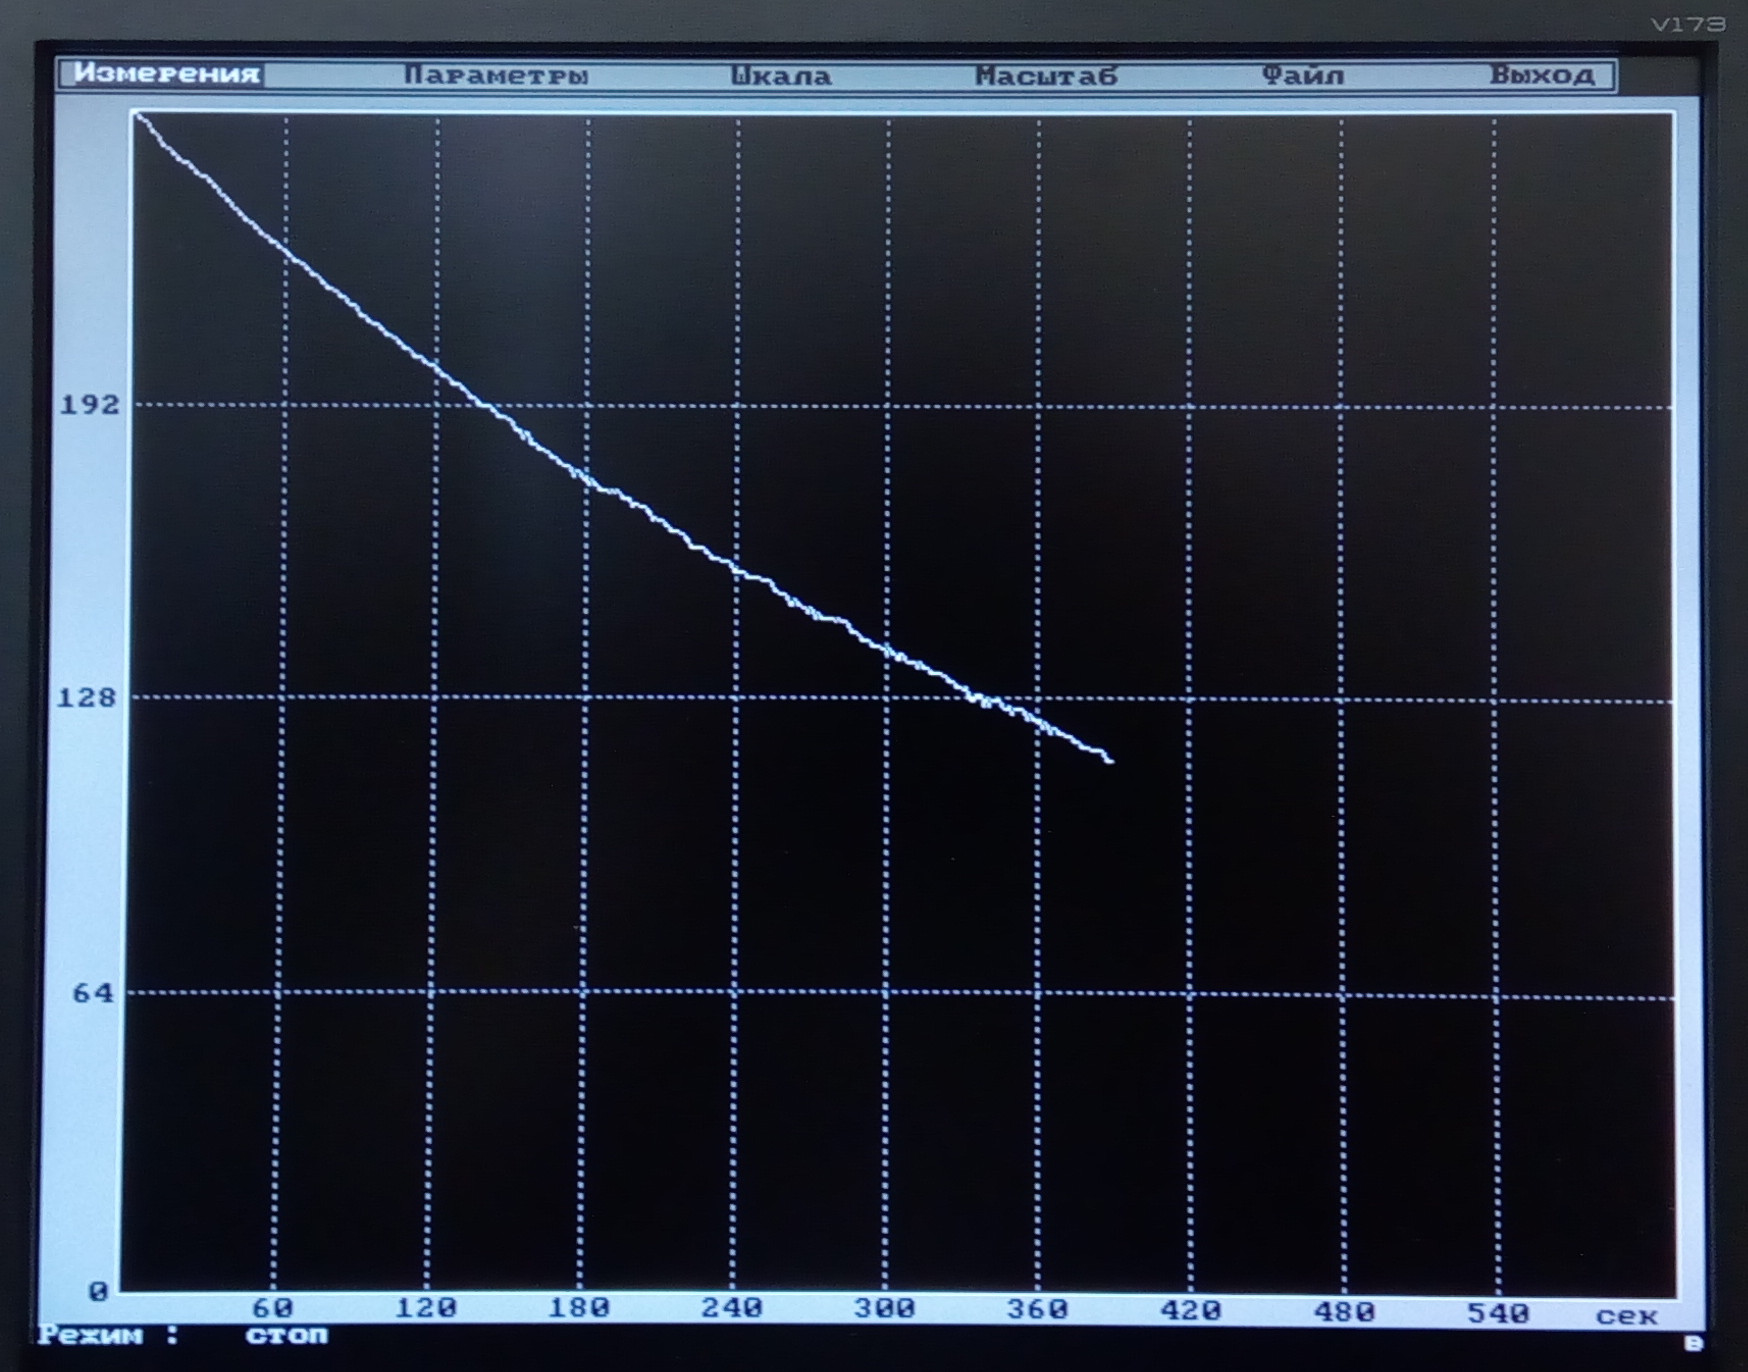
\includegraphics[scale=0.14]{graph-40t.jpg}
		\end{minipage}
		\begin{minipage}{0.49\linewidth}
			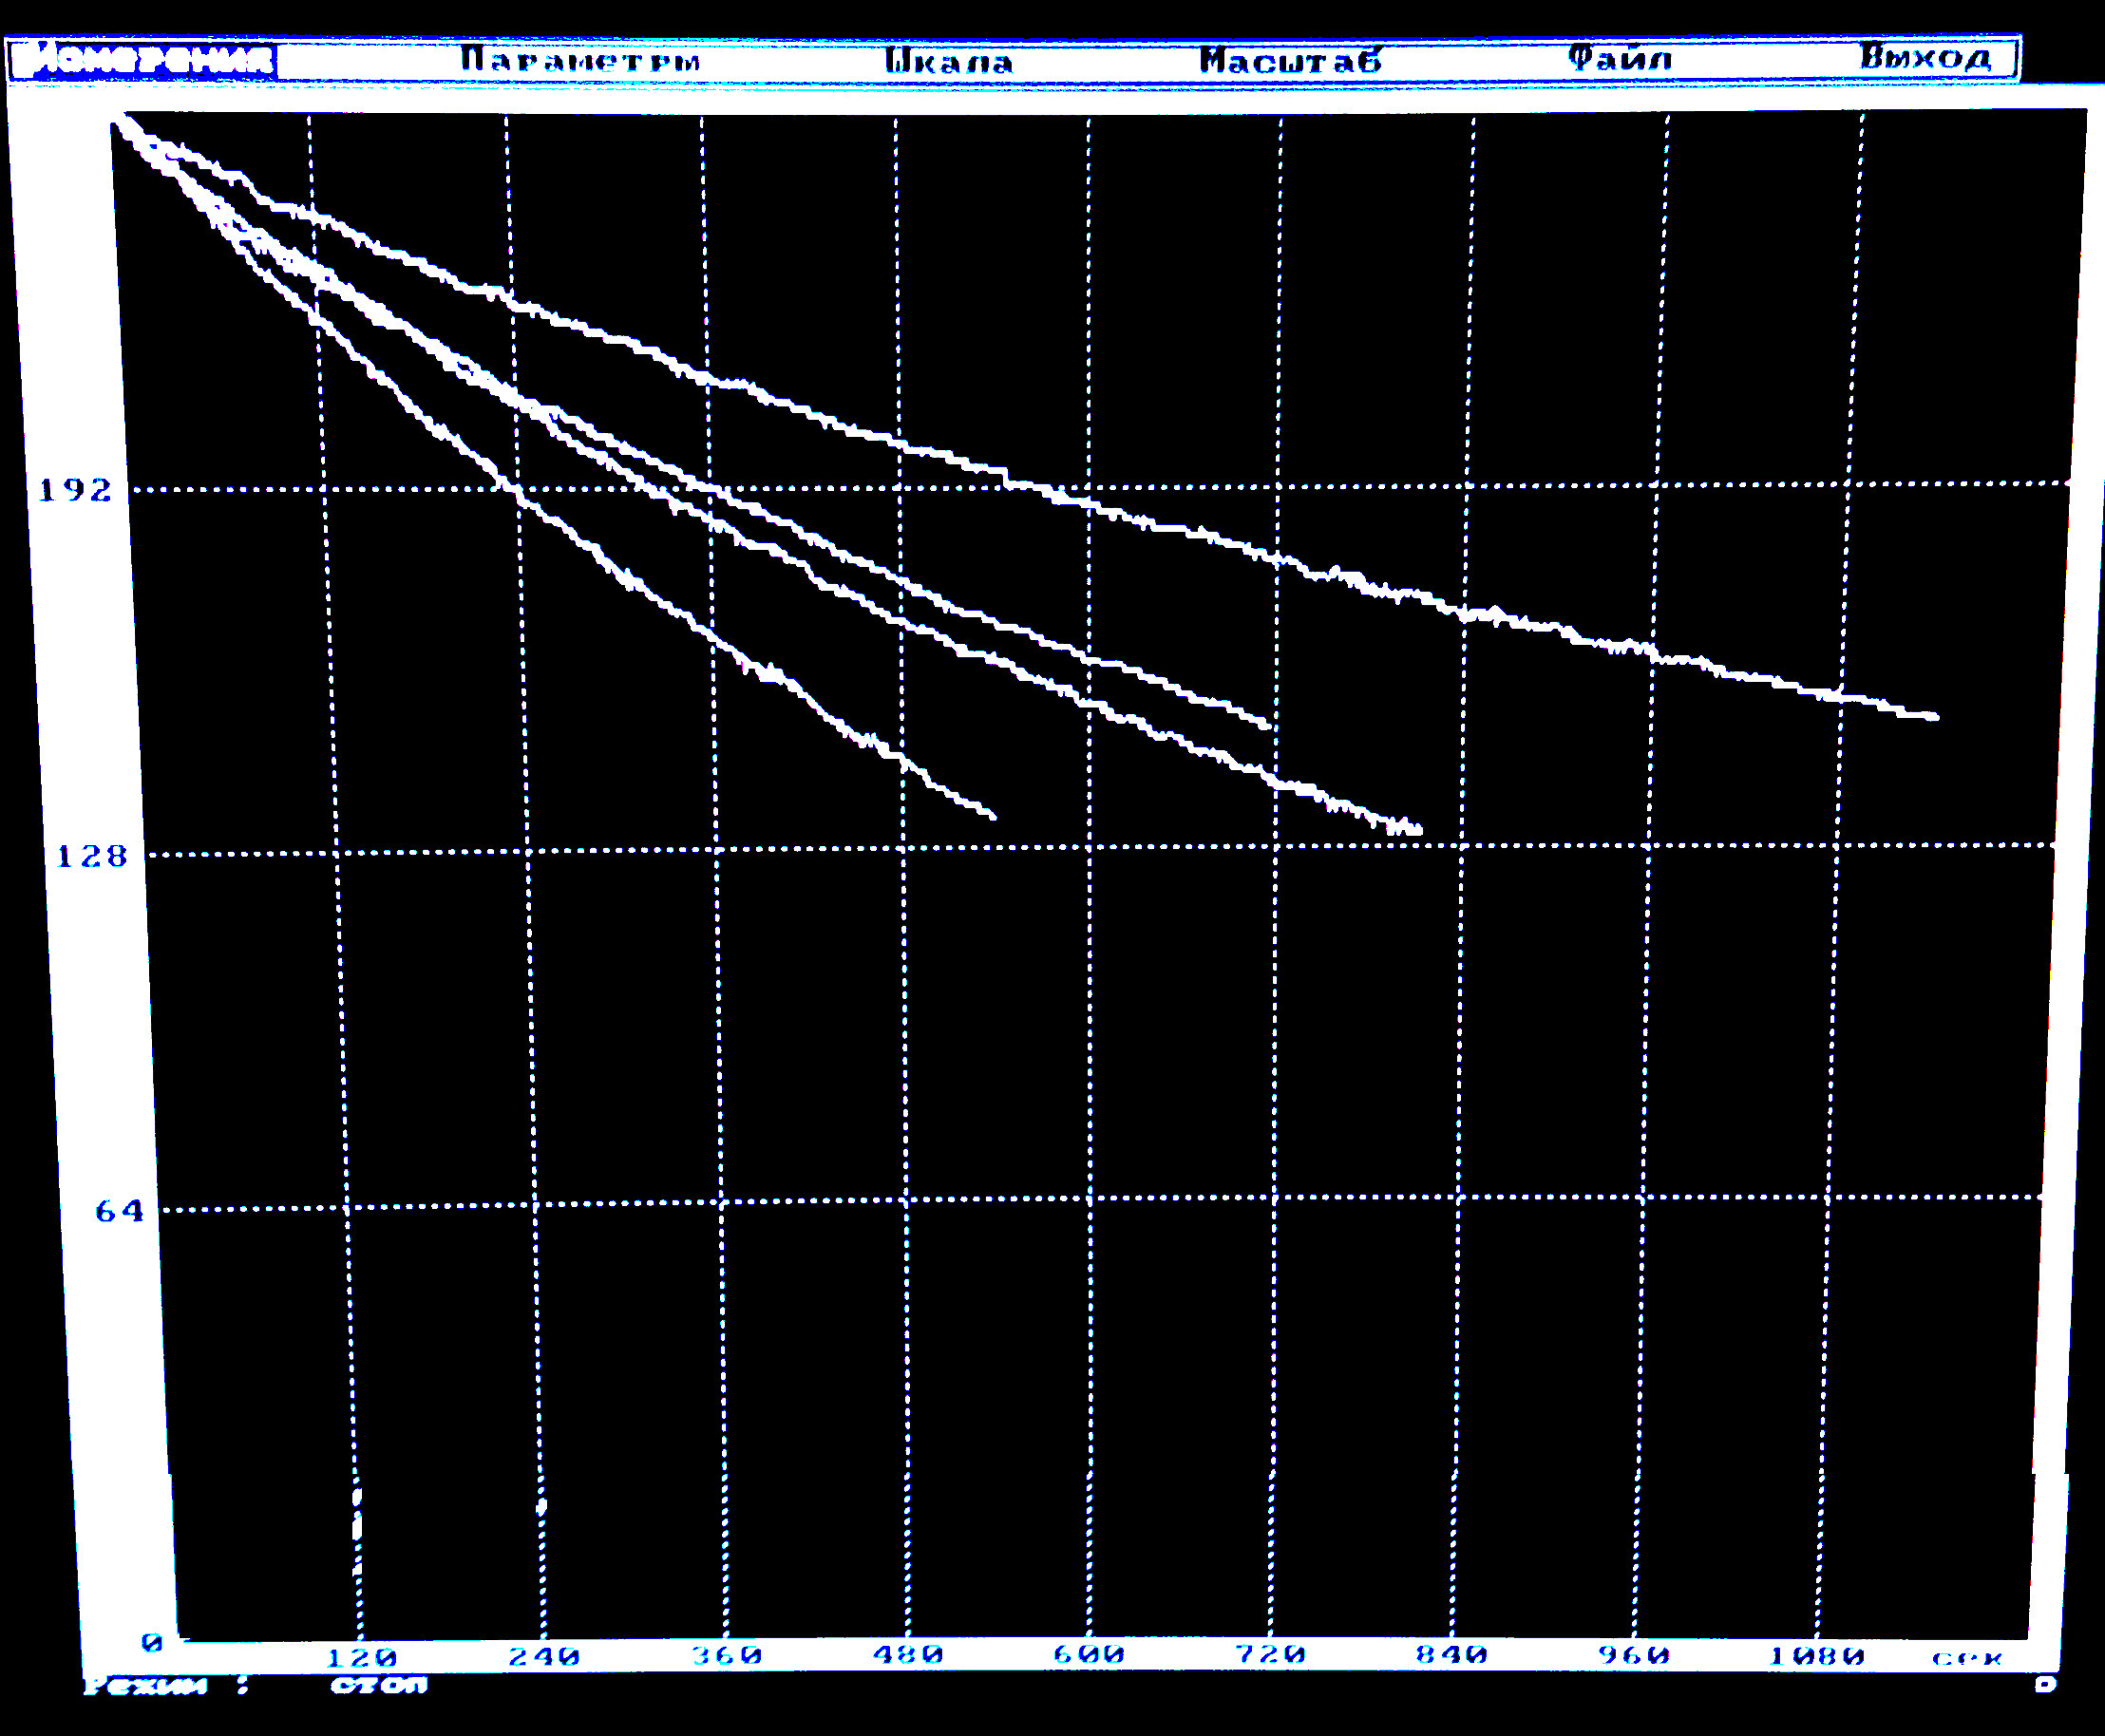
\includegraphics[scale=0.105]{graph-all.jpg}
		\end{minipage}
	\end{figure}
	
	К сожалению, после снятия измерений для 40 торр компьютер завис, так что логарифмического графика не сохранилось. Остальные приведены на \fref{graphs-log}, чем выше график, тем ниже давление.
	
	\begin{figure}[!h]
		\caption{Графики $N(t)$ в логарифмическом масштабе}
		\begin{center}
		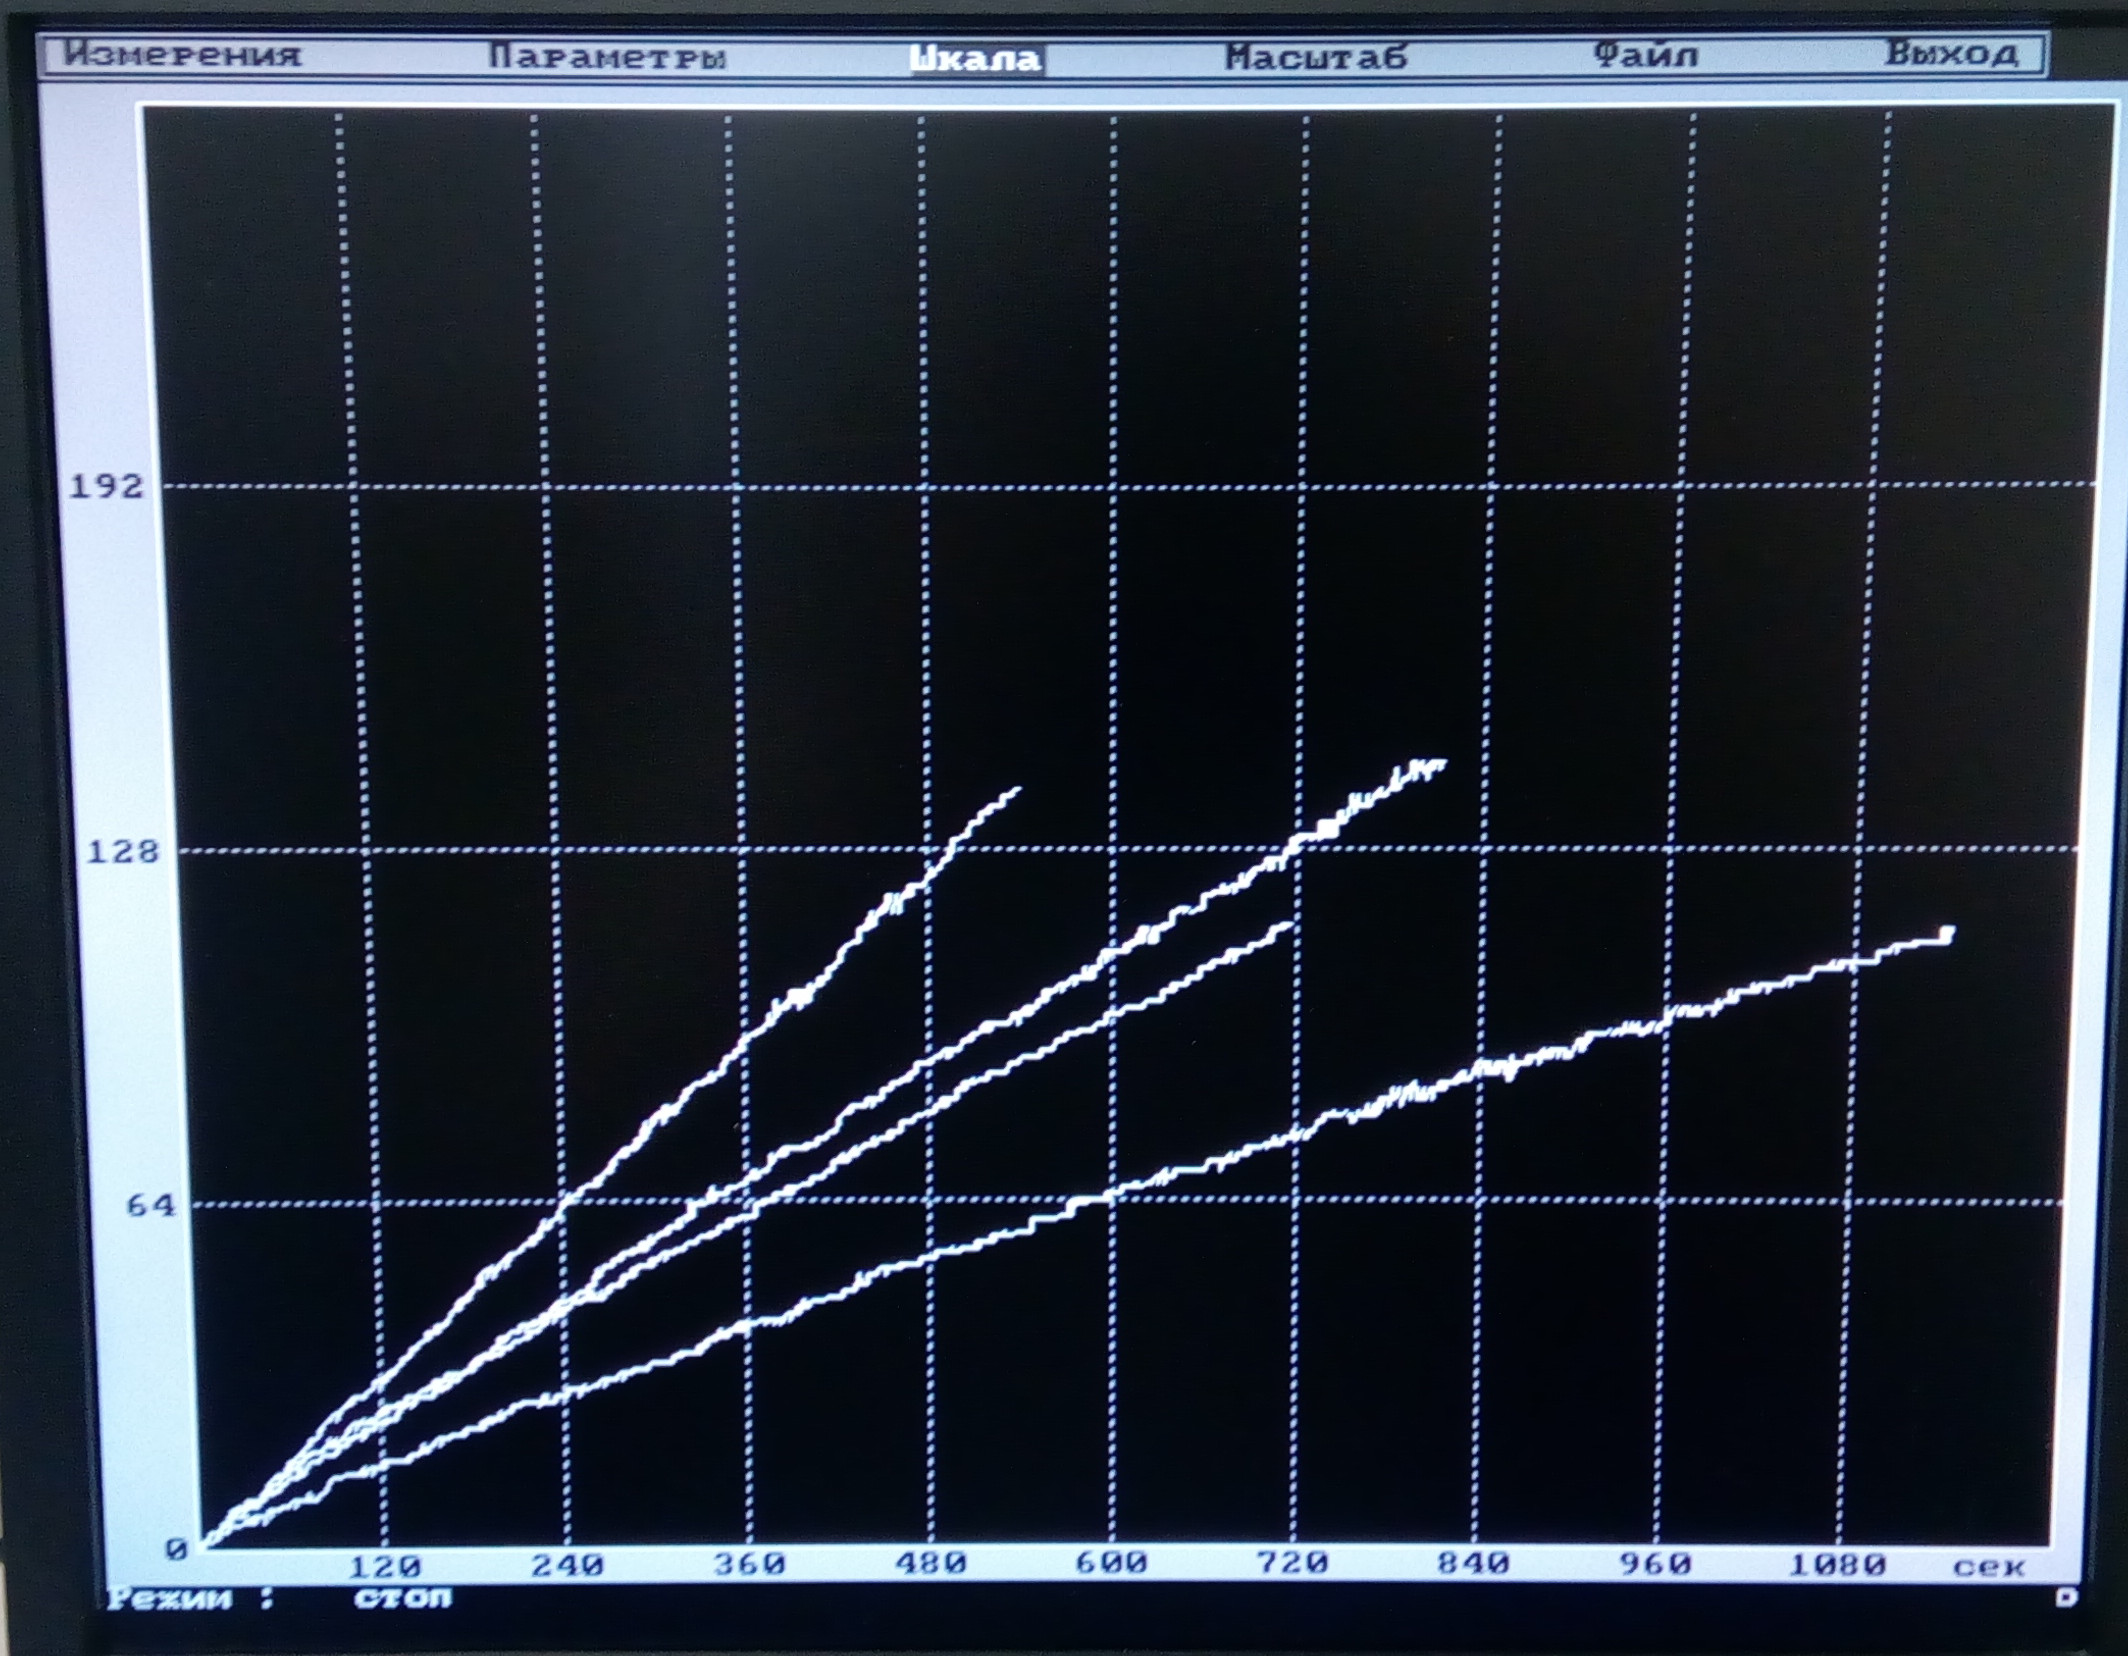
\includegraphics[scale=0.1]{graph-all-log.jpg}
		\end{center}
		\label{graphs-log}
	\end{figure}
	
	На компьютере по введенным параметрам установки были рассчитаны коэффициенты диффузии и их погрешности для всех температур, они приведены в таблице \ref{tb:diffusion_co}
	
	\begin{table}[!h]
		\caption{Коэффициенты диффузии для разных давлений}
		\label{tb:diffusion_co}
		\begin{center}
			\begin{tabular}{|c|c|c|c|}
				\hline
				$P$, торр & $D$, $\frac{\text{см}^2}{\text{с}}$ & $\sigma_D/D$ & $\sigma_D$, $\frac{\text{см}^2}{\text{с}}$ \\
				\hline
				40 & 9,1 & 0,098 & 0,9 \\
				80 & 5,3 & 0,098 & 0,5 \\
				120 & 3,7 & 0,104 & 0,4 \\
				160 & 3,2 & 0,133 & 0,4 \\
				250 & 2,0 & 0,125 & 0,3 \\
				\hline
			\end{tabular}
		\end{center}
	\end{table}
	
	Затем я построил график $D(1/P)$ (\fref{graph-DP}).
	
	\begin{figure}[!h]
		\caption{График $D(1/P)$}
		\begin{center}
		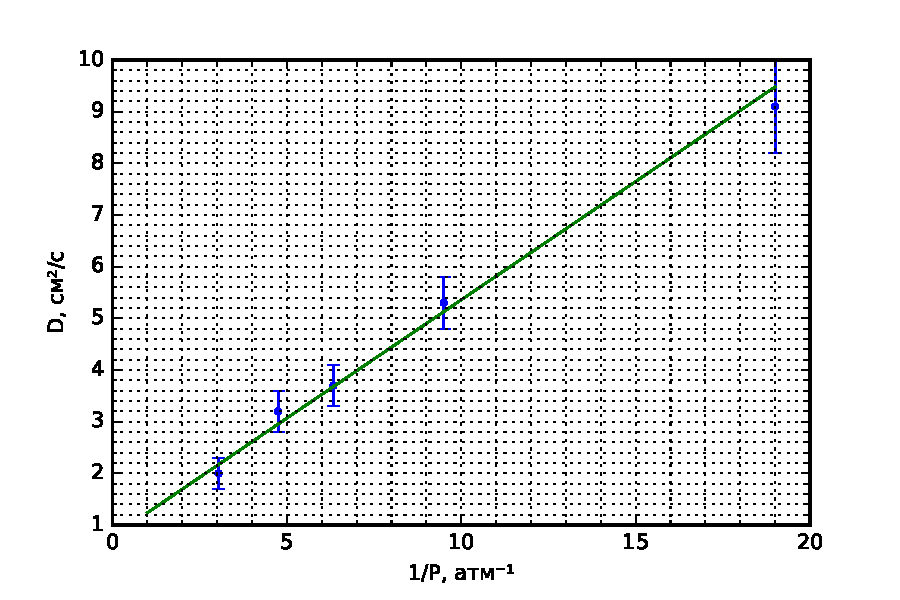
\includegraphics[scale=.8]{graph-DP.pdf}
		\end{center}
		\label{graph-DP}
	\end{figure}
	
	Я линейно аппроксимировал его как $D=D_0+K/P$ и получил следующие значения: $$ D_0=(0{,}8\pm 0{,}2) \frac{\text{см}^2}{\text{с}}, $$ $$ K=(0{,}46\pm 0{,}03) \frac{\text{см}^2 \cdot \text{атм}}{\text{с}}. $$
	
	По этим коэффициентам я нашёл коэффициент диффузии при атмосферном давлении: $$ D_\text{атм}=(1{,}2\pm 0{,}2) \frac{\text{см}^2}{\text{с}}. $$
	
	Табличное значение из лабника для воздуха и гелия при $0\degC$: $D=0{,}62 \frac{\text{см}^2}{\text{с}}$. Оно отличается от полученного в два раза, причина, скорее всего, в том, что они при разных температурах.
	
	Оценим длину свободного пробега и размер молекулы, считая, что взаимная диффузия обеспечивается в основном гелием.
	По формуле для коэффициента диффузии
	\begin{equation}
		\label{eq:diff_co_fla}
		D=\frac{1}{3} \bar{v} \lambda.
	\end{equation}
	
	Как известно, средняя скорость
	\begin{equation}
		\label{eq:v_avg}
		\bar{v} = \sqrt{\frac{8RT}{\pi \mu}}
	\end{equation}
	
	В свою очередь, длина свободного пробега определяется из условия
	\begin{equation}
		\label{eq:lambda_fla}
		\pi n d^2 \lambda=1,
	\end{equation}
	при этом
	\begin{equation}
		\label{eq:press_fla}
		P=nkT.
	\end{equation}
	
	Результаты оценок приведены в таблице \ref{tb:lambda_d}
	
	\begin{table}[!h]
		\caption{Длина свободного пробега и размер молекулы для разных давлений}
		\label{tb:lambda_d}
		\begin{center}
			\begin{tabular}{|c|c|c|}
				\hline
				$P$, торр & $\lambda$, мкм & $d$, \AA \\
				\hline
				40 & 2 & 3 \\
				80 & 1 & 3 \\
				120 & 0,9 & 3 \\
				160 & 0,7 & 3 \\
				250 & 0,5 & 3 \\
				760 & 0,3 & 2 \\
				\hline
			\end{tabular}
		\end{center}
	\end{table}
	
\end{document}
